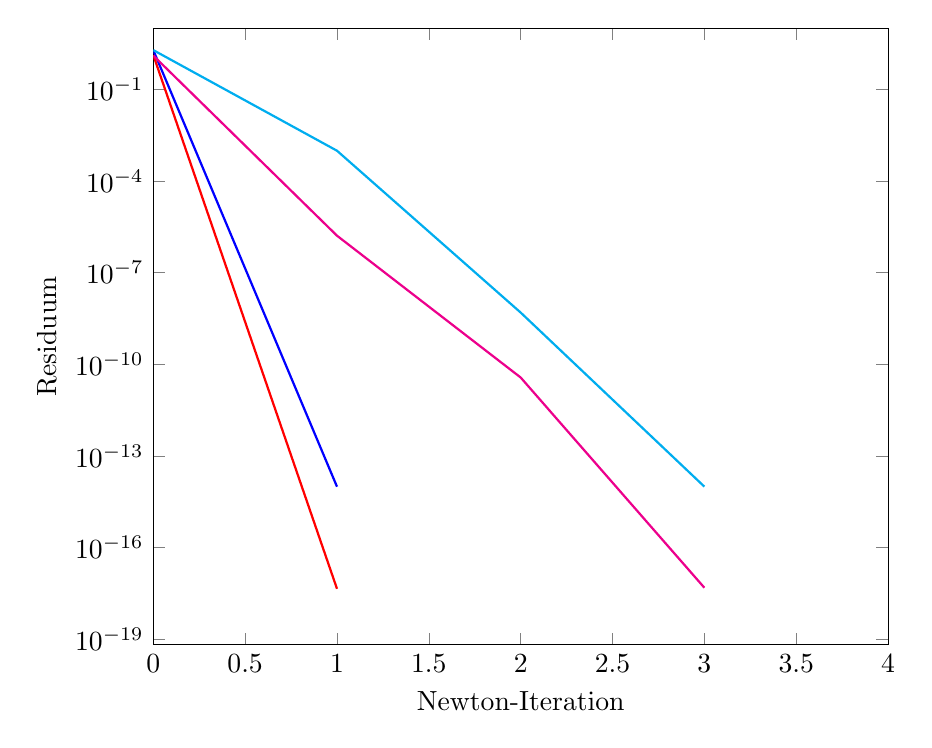
\begin{tikzpicture}[every plot/.append style={thick}] 
\begin{axis}[ 
label style={font=\normalsize}, 
xlabel={Newton-Iteration}, 
ylabel={Residuum}, 
xmin=0, xmax=4, 
ymode=log, 
ymin=0, ymax=10, 
width=0.9\textwidth, 
grid style=dashed, 
] 
\addplot[ 
color=blue, 
] 
coordinates { 
(0, 1.91e+00)(1, 9.86e-15)}; 
\addplot[ 
color=red, 
] 
coordinates { 
(0, 1.32e+00)(1, 4.49e-18)}; 
\addplot[ 
color=cyan, 
] 
coordinates { 
(0, 1.92e+00)(1, 9.78e-04)(2, 4.93e-09)(3, 9.90e-15)}; 
\addplot[ 
color=magenta, 
] 
coordinates { 
(0, 1.27e+00)(1, 1.62e-06)(2, 3.69e-11)(3, 4.86e-18)}; 
\end{axis} 
\end{tikzpicture} 
